%%%%%%%%%%%%%%%%%%%%%%%%%%%%%%%%%%%%%%%%%%%%%%%%%%%%%%%%%%%%%%
\chapter{Model Inspection and Reproduction}
\label{app:model_inspection}
%%%%%%%%%%%%%%%%%%%%%%%%%%%%%%%%%%%%%%%%%%%%%%%%%%%%%%%%%%%%%%

This appendix separates visual process inspection from executable
reproduction. The complete directly-follows graph exposes every observed
training-log relation, while the handover package contains the Petri net and
the exact simulation-parameter bundles used for the reported baseline and
what-if scenarios. The graph is descriptive. The PNML and serialized ProSiT
objects are the executable models.

\section{Unfiltered Training-Log Control Flow}

Figure~\ref{fig:appendix_full_dfg} shows the unfiltered 59-arc directly-follows
graph of the order-preserving training log. It is included for audit because
the dominant-frequency view in Chapter~\ref{chp:experiments_and_framework}
deliberately suppresses rare relations. The complete view confirms the fixed
gate boundary and makes low-frequency repetitions and cross-activity relations
inspectable. Its density also demonstrates why it is unsuitable as the primary
explanatory figure. It should not be interpreted as a Petri net. In particular,
a directly-follows arc records observed succession but does not encode choice,
concurrency, markings, or firing rules.

\begin{sidewaysfigure}[p]
\centering
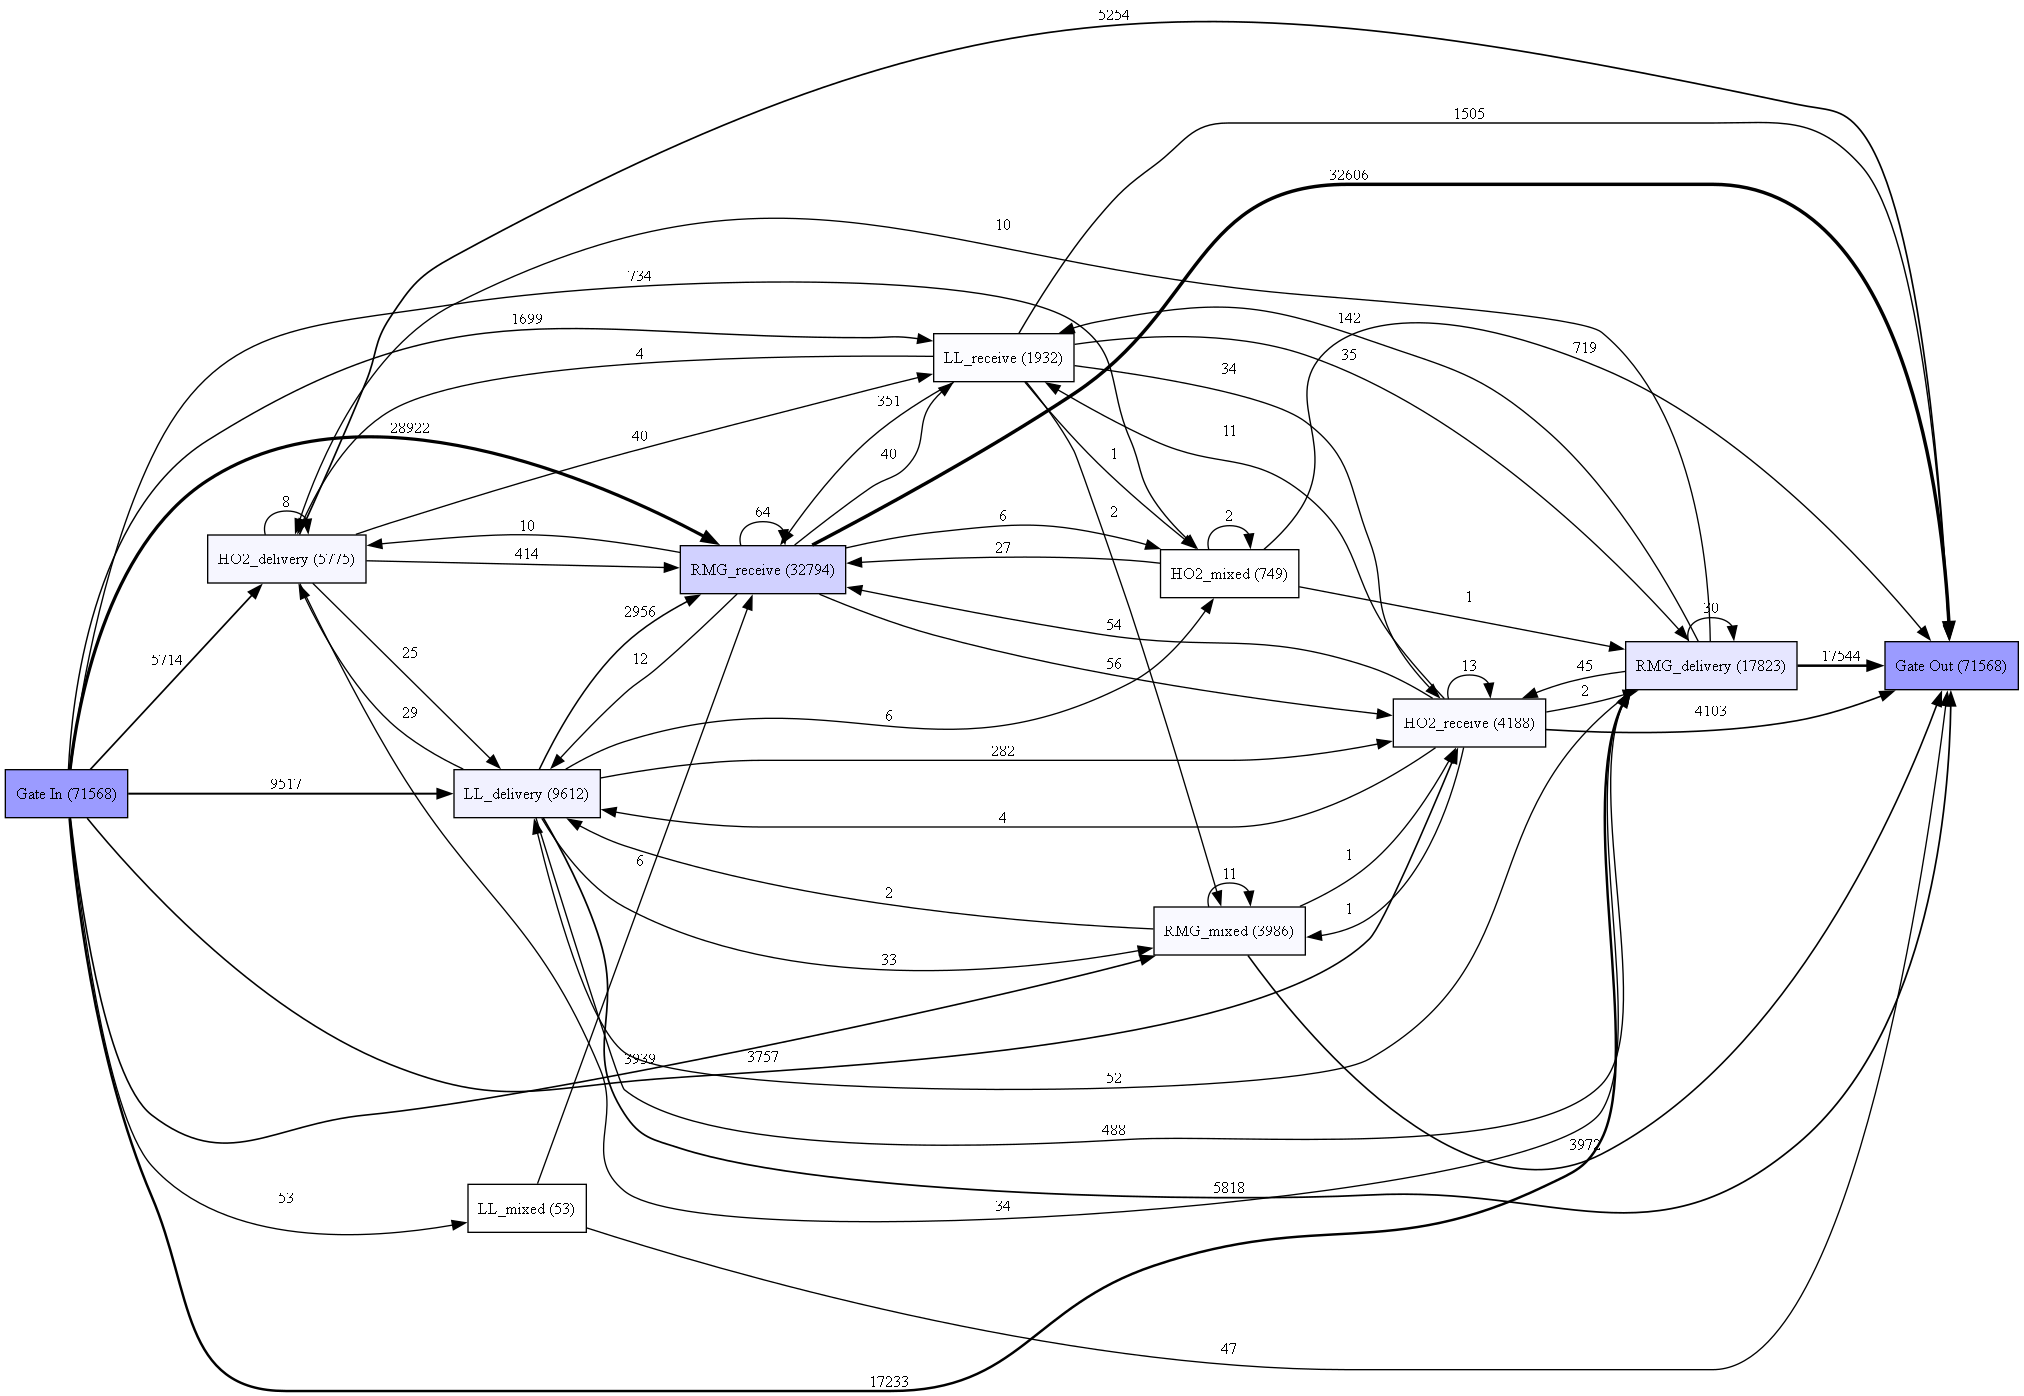
\includegraphics[width=0.92\textheight,height=0.88\textwidth,keepaspectratio]{figures/discovery/dfg_frequency_inductive_training.png}
\caption{Complete frequency directly-follows graph of the order-preserving CTB
training log. Node labels report activity occurrences and arc labels report
directly-follows counts. All 59 observed arcs are retained. The figure is a
descriptive audit view and is not the executable simulation model.}
\label{fig:appendix_full_dfg}
\end{sidewaysfigure}

\section{Executable Model Artifacts}

The independently uploadable folder \texttt{CTB\_ProSiT\_reproduction}
contains the minimal reviewer handover. Table~\ref{tab:appendix_model_artifacts}
maps each file to its role. The baseline and both scenario bundles are separate
serialized objects. They therefore allow inspection of the actual model state
rather than relying on parameter values transcribed into the manuscript.

\begin{table}[htbp]
\centering
\begin{tabularx}{\textwidth}{L{5.2cm}X}
\toprule
\textbf{Artifact} & \textbf{Role in inspection and reproduction} \\
\midrule
\texttt{models/ctb\_inductive\_miner.pnml} & Common discovered Petri net with its executable control-flow structure. \\
\texttt{models/params\_baseline.pkl} & Exact cap-three \textit{visit-only} baseline object used by the scenario runner. \\
\texttt{models/params\_t22\_closed.pkl} & Scenario A object with T22 removed from the eligible RMG resource pool and calendar. \\
\texttt{models/params\_demand\_plus\_20pct.pkl} & Scenario B object with the working-time inter-arrival samples scaled to increase configured demand by 20\,\%. \\
Corresponding \texttt{.json} files & Human-readable parameter descriptions for inspecting rules, distributions, resources, calendars, and scenario changes. \\
\texttt{expected\_results/} & Reference result tables used to check that a completed run reproduces the thesis outputs. \\
\texttt{CTB\_ProSiT\_Local.ipynb} and \texttt{CTB\_ProSiT\_Colab.ipynb} & Minimal local and Google Colab entry points that load the frozen models, run the simulations, and compare the generated results with the reference files. \\
\texttt{PROVENANCE.json}, \texttt{README.md}, and \texttt{requirements.txt} & File hashes, model roles, execution instructions, and the required software environment. \\
\bottomrule
\end{tabularx}
\caption{Reviewer-handover artifacts for model inspection and result reproduction.}
\label{tab:appendix_model_artifacts}
\end{table}

The public ProSiT save-and-load workflow serializes discovered parameters so
that simulation can be repeated without rerunning discovery
\cite{ProSiTRepository}. The handover follows that workflow and additionally
retains the exact Python objects used for the CTB experiments. The JSON files
are important because they expose the fitted model in a portable and readable
form. The pickles remain the execution source for the reported numbers because
the CTB calibration uses empirical sample arrays whose exact runtime state is
not completely represented by the JSON companions. Pickles must only be loaded
from this trusted handover and with the recorded environment.

The reviewer opens one notebook and executes its cells from top to bottom. The
notebook loads the PNML together with the baseline and both scenario bundles,
runs the same trace count and seeds used in the thesis, writes generated result
tables to a new output directory, and compares them with
\texttt{expected\_results}. No discovery or manual model reconstruction is
required. The local notebook uses the packaged Python environment. The Colab
required. The local notebook installs the pinned requirements into the active
Jupyter environment. The Colab notebook creates an isolated Python 3.11
environment and installs the same pinned requirements before loading the
artifacts. This keeps the manuscript focused on experimental logic while
making the complete executable state available to an interested reader.
